\documentclass[tikz,border=2pt]{standalone}
\usepackage{amsmath}
\usetikzlibrary{arrows.meta}
\begin{document}
% Separation X <=_st Y <=_sl Z with E[Y] = E[Z]: X = 0 surely, Y = 1 surely, Z in {0,2} with probability 1/2 each.
% Step 1 moves the mass up (stochastic order); step 2 spreads it at the common mean 1 (convex order).
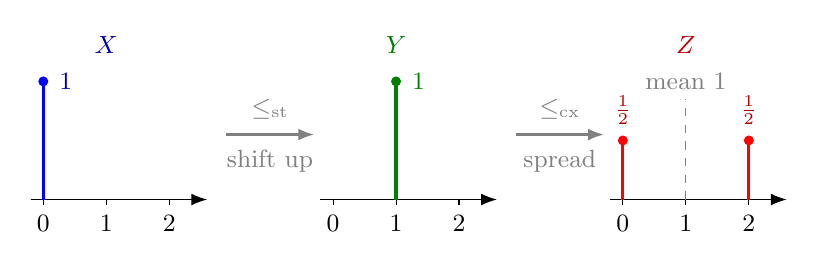
\begin{tikzpicture}[font=\small, >={Latex[length=2mm]}, x=0.8cm, y=1.5cm]
  % one probability-mass panel per law: axis from 0 to 2.5 with ticks 0,1,2
  \foreach \ox/\nm/\col in {0/X/blue!70!black, 4.6/Y/green!50!black, 9.2/Z/red!70!black} {
    \begin{scope}[xshift=\ox*0.8cm]
      \draw[->] (-0.2,0) -- (2.6,0);
      \foreach \t in {0,1,2} {\draw (\t,0) -- (\t,-0.05) node[below] {$\t$};}
      \node[anchor=south, text=\col] at (1,1.15) {$\nm$};
    \end{scope}
  }
  % X = 0
  \draw[blue, very thick] (0,0) -- (0,1); \fill[blue] (0,1) circle (1.8pt);
  \node[blue!70!black, anchor=west] at (0.1,1) {$1$};
  % Y = 1
  \draw[green!50!black, very thick] (5.6,0) -- (5.6,1); \fill[green!50!black] (5.6,1) circle (1.8pt);
  \node[green!50!black, anchor=west] at (5.7,1) {$1$};
  % Z in {0,2}
  \draw[red, very thick] (9.2,0) -- (9.2,0.5); \fill[red] (9.2,0.5) circle (1.8pt);
  \draw[red, very thick] (11.2,0) -- (11.2,0.5); \fill[red] (11.2,0.5) circle (1.8pt);
  \node[red!70!black, anchor=south] at (9.2,0.55) {$\tfrac12$};
  \node[red!70!black, anchor=south] at (11.2,0.55) {$\tfrac12$};
  % common mean of Y and Z
  \draw[gray, thin, dashed] (10.2,0) -- (10.2,0.85);
  \node[gray, anchor=south] at (10.2,0.85) {mean $1$};
  % the two steps
  \draw[->, thick, gray] (2.9,0.55) -- (4.3,0.55);
  \node[gray, anchor=south] at (3.6,0.6) {$\le_{\mathrm{st}}$};
  \node[gray, anchor=north] at (3.6,0.5) {shift up};
  \draw[->, thick, gray] (7.5,0.55) -- (8.9,0.55);
  \node[gray, anchor=south] at (8.2,0.6) {$\le_{\mathrm{cx}}$};
  \node[gray, anchor=north] at (8.2,0.5) {spread};
\end{tikzpicture}
\end{document}
